\chapter{Pseudo Random Number Generation}
\section{Producing binomial random variables}

The exercise is about different methods to produce pseudo random numbers with different distributions. One can do it in several ways to get pseudo random numbers. Most of methods use uniform distributed variables in some way or other. We don't consider the process of simulating uniformly distributed variables here. There are different methods, like Whichmann-Hill or the LCG, that are provided by R. 

\noindent
One easy way to get random simulations of a specific distribution is by using uniformly distributed variables and the quantile transformation of the desired distribution. In the first part of the exercise we simulate binomial random variables using this idea. The second part is about the accept-reject method to simulate standard normal random variables.

The inversion method is based on the generalised inverse of the distribution function (cdf) $F$ which is considered to be defined on $\RR$ here and its inverse defined on $t \in (0, 1)$ as
$$F^{-1}(t) = inf\{x \in \RR | F(x) \geq t\}.$$
This, requires that the cdf is in this way analytical invertible. Additionally, if $U \sim unif[0, 1]$ holds, then $F^{-1}(U) \sim F$, i.e., it is possible to generate $F$-distributed variables using uniform variables.

In this exercise we were asked to simulate binomial random variables with parameters $n = 10$ and $p = 0.4.$ The inverse is easily computed as a sum of indicator functions over the intervals $[0,B(n,p)(\{k\})]$ for $k = 0, \dots 10.$ So we produced $1000$ binomials using the inverse of simulated uniforms. Another way to get binomial distributed variables is the summation of independent Bernoulli random variables with success
probability $p.$ Those can also be simulated using the inverse method with $F^{-1}(t) = \one_{[0,p)}(t).$ Therefore we used in another trial $10000$ uniform distributed variables that we inverted to Bernoulli variables and added up in the end. Finally we compared those
two approaches with the provided method \texttt{rbinom} which is based on a special accept-
reject-method. In the visualisation we can see very clear that all approaches lead to
a similar distribution (see Figure \ref{fig:emp_all}). Although the binomial distribution is discrete, I have added a smooth density estimate to compare the overall shape of the distributions.

\begin{figure}[th]
\centering
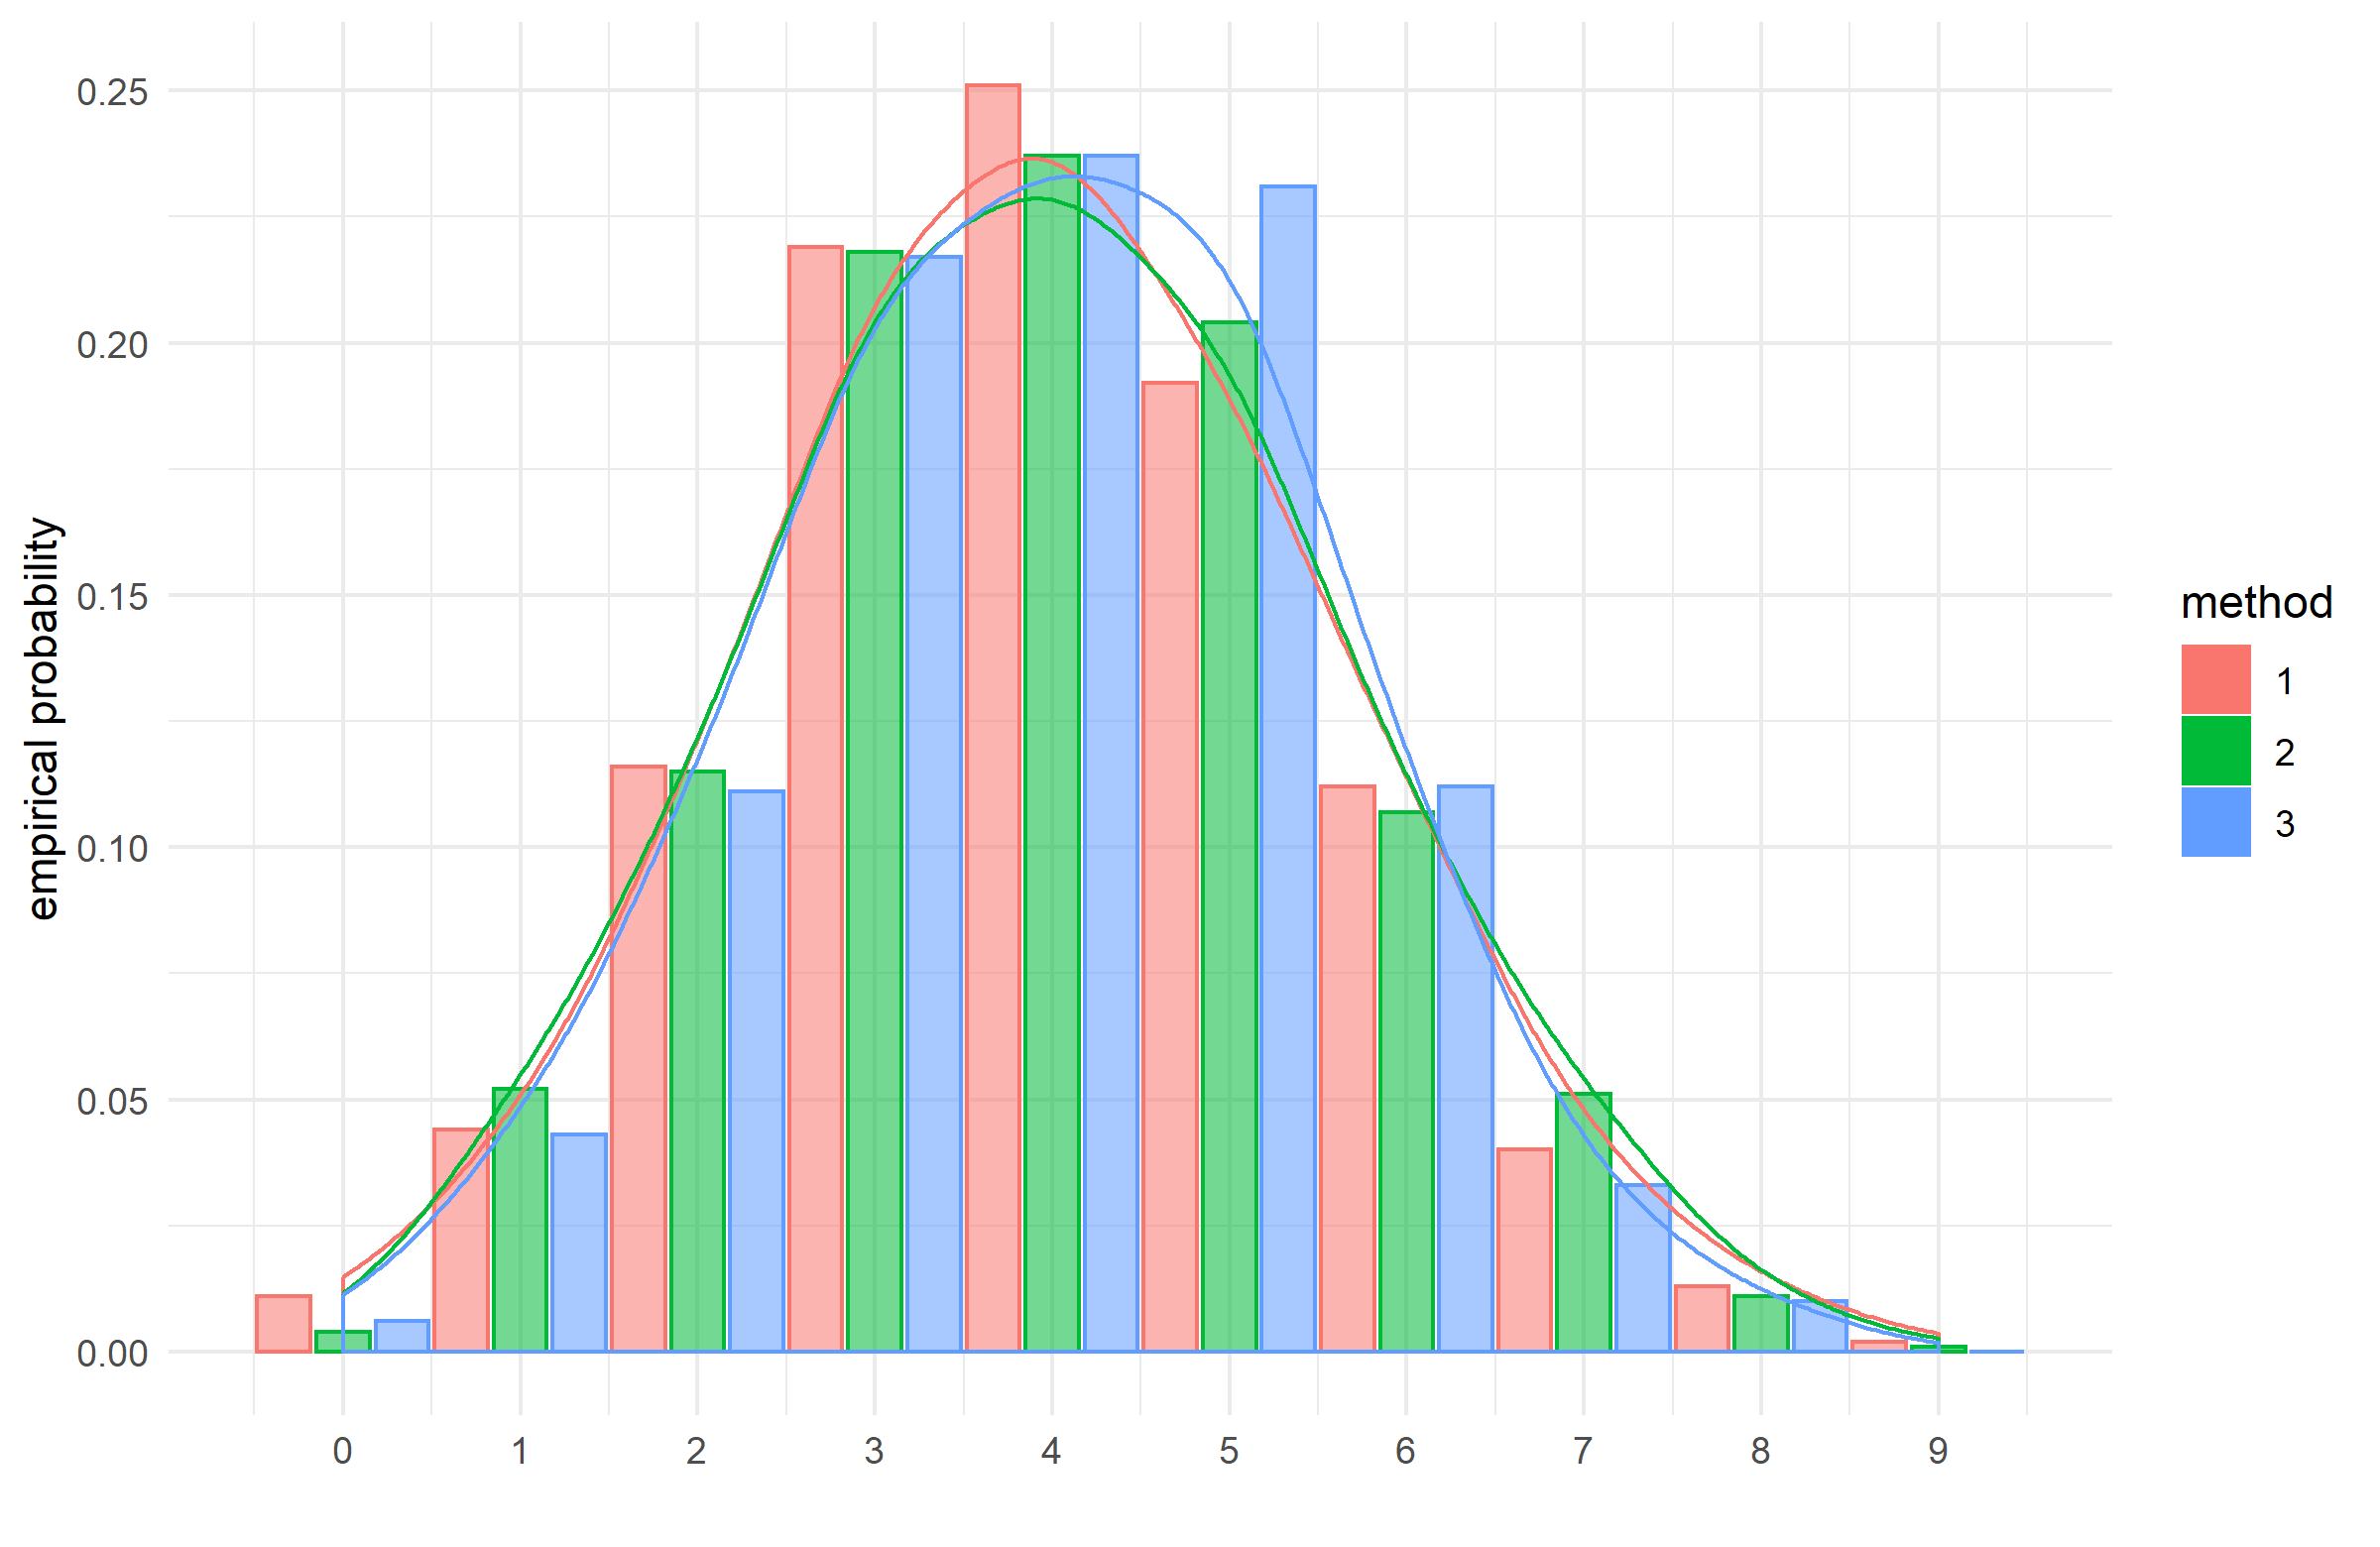
\includegraphics[scale = 0.7]{ex2/emp_all.png}
\caption{Empirical distribution of simulated binomial variables ($n=10, p=0.4$). Method 1: inverse method with the binomial quantile function; \\
Method 2: Summation of Bernoulli variables (simulated with uniform variables and inverse method);\\
Method 3: simulated with \texttt{rbinom}.}
\label{fig:emp_all}
\end{figure}  

So we see that the first two method, i.e. those using inverse method just differ in a slightly more centred distribution for method $1$. The blue bins show a small shift of the distribution to the right most dominant at $5.$

Drawing a histogram of three groups into one plot is sometimes problematic because the bins are drawn shifted in a graphical way. This shift may suggest a shift in distribution that is not existent in the data. Therefore I have added another graphic (Figure \ref{fig:emp_all_col}) where I put the three histograms beneath each other. As the three distributions are very close, in general differences are hard to see, but one sees that method $1$ generates a more centred distribution and that the first row shows a slightly more right skewed distribution, as one would expect from a binomial with $p=0.4$. All in all the differences seem somehow negligible and we can assume that every method produced reasonable simulations.

\begin{figure}[thbp]
\centering
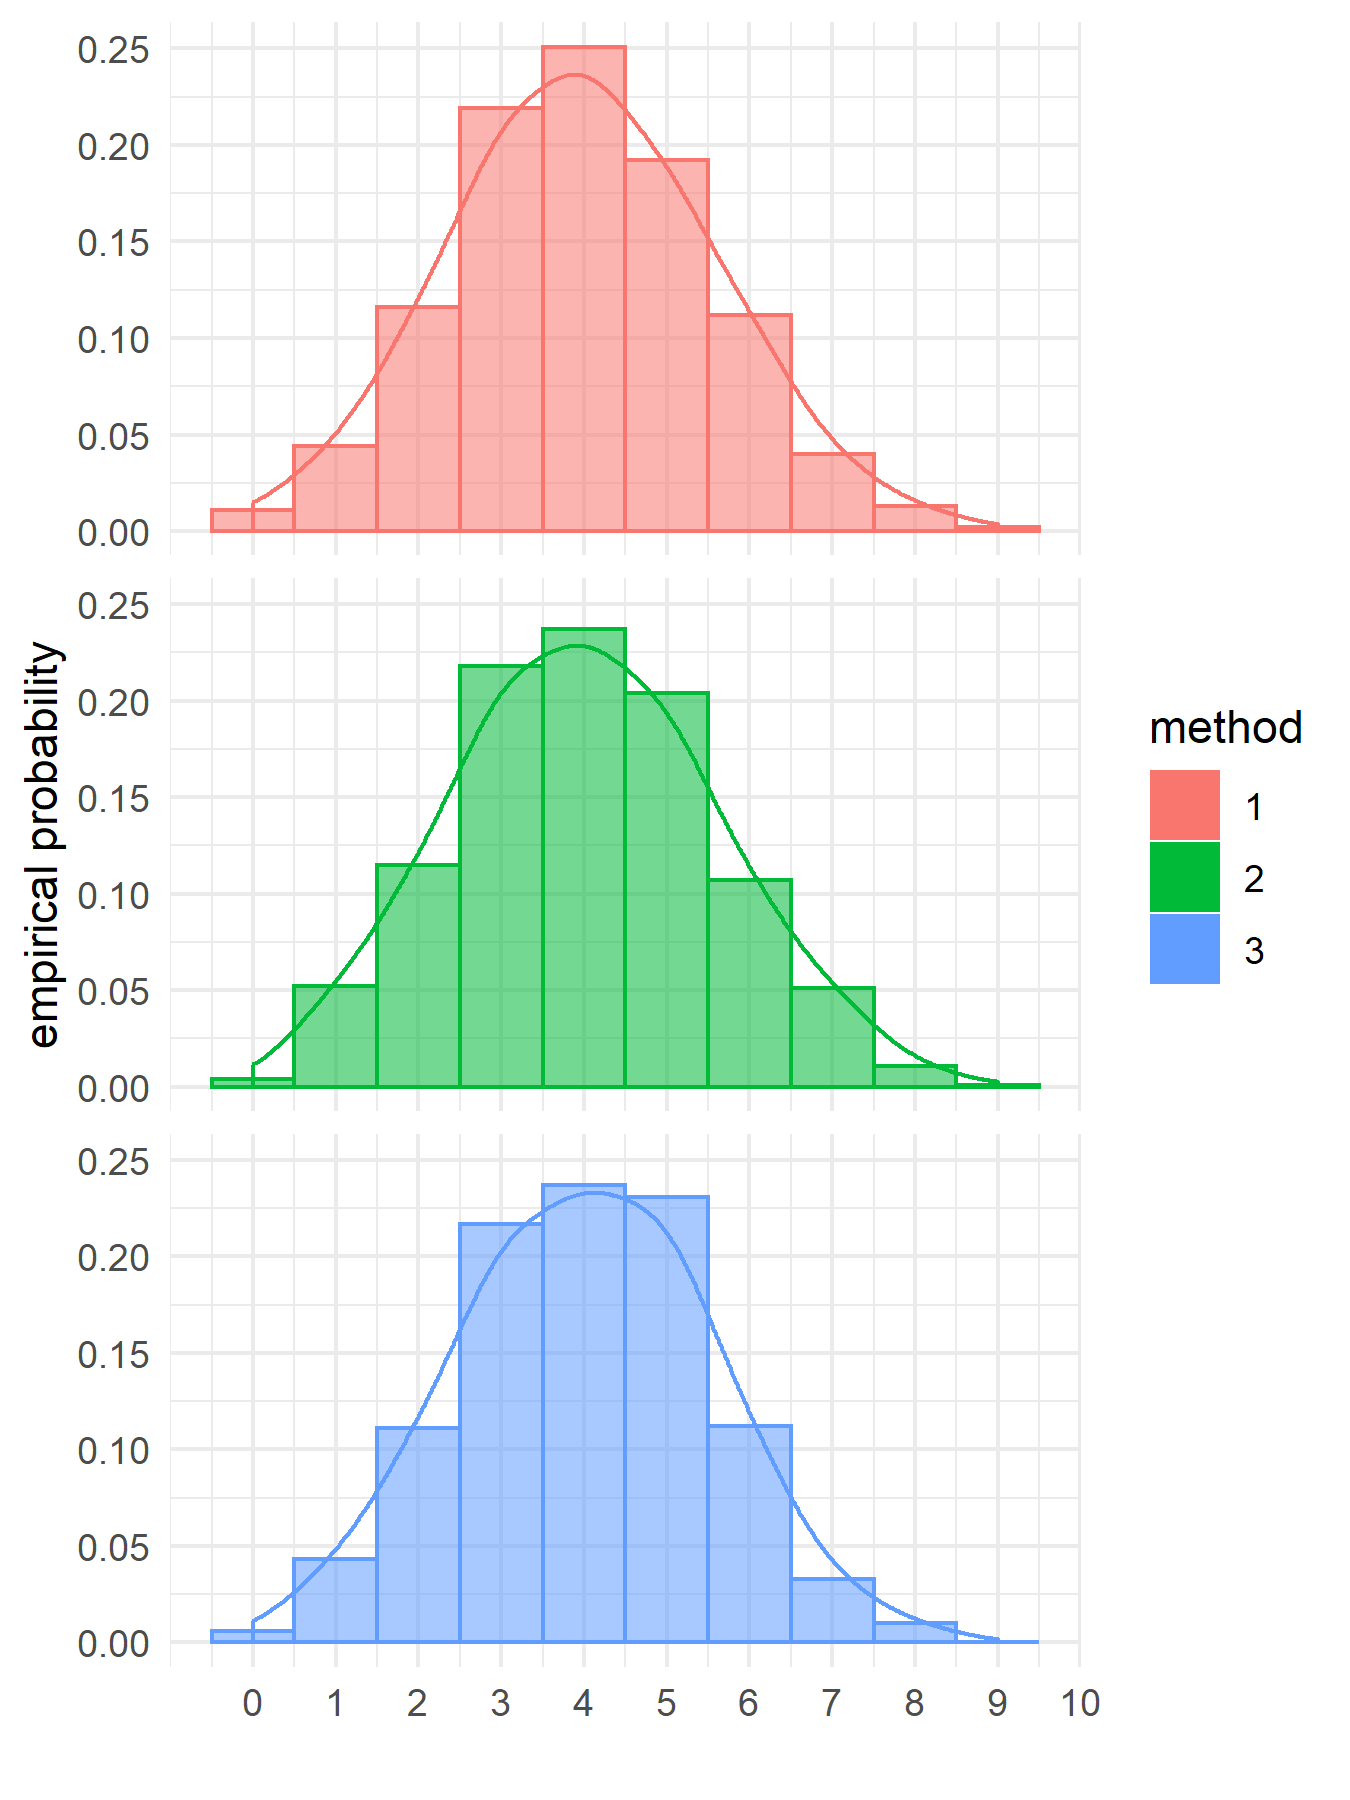
\includegraphics[scale = 0.8, keepaspectratio]{ex2/emp_all_col.png}
\caption{Histograms of simulated binomial variables with the three methods.}
\label{fig:emp_all_col}
\end{figure}

\newpage
\section{Accept-reject method for normal distribution}

The next task is to produce standard normal random variables with the accept-reject method. Therefore one has to be able to simulate variables from another distribution with known density. Here we use the standard Cauchy distribution with the density $g(x)=[\pi (1+x^2)]^{-1}$.\\

The general approach for generating variables with a density function $f$ by variables with a distribution given by a density $g$ demands a constant $c\geq 1$, s.t. $f(x)\leq cg(x)$ for all $x$ and is given by following algorithm:
\begin{enumerate}
\item generate random variable $X$ from density $g$
\item generate uniformly distributed $U\sim unif[0,1]$ (independent from $X$)
\item Accept $X$ as drawn from $f$, if $Ucg(X)\leq f(X)$, else reject.
\end{enumerate} 

The resulting variables $X$ are then distributed with density $f$. In this exercise we produce the variables $X$ with the inversion method. The cdf of the standard Cauchy distribution is given by $$G(x)= (\arctan (x) - 0.5)/\pi$$ and therefore we get the inverse $$G^{-1}(t)=\tan \{\pi (y-0.5)\}.$$

To determine the best $c$ for the rejection procedure, we search for the smallest possible constant - as we don't want to reject unnecessary many $X$ so we have to draw less candidates and thus keep the algorithm fast - such that $c\geq \frac{f}{g}(x)$ for all $x$, i.e. $$c:= \sup_{x\in \mathbb{R}} \frac{f(x)}{g(x)}= \sup_{x\in \mathbb{R}} \frac{1}{\sqrt{2\pi}}\exp\{-x^2/2\} \pi (1+x^2).$$ By differentiation we get three local extrema and the maxima at $x\in \{-1,1\}$ resulting in $c=\sqrt{2\pi}e^{-1/2}$.

We simulated $10,000$ standard normals using this method after setting the random number generator back to default, i.e. using Mersenne-Twister. The result is shown in Figure \ref{2normhist}. There we can see a very good fit of the data.
\begin{figure}[!th]
\centering
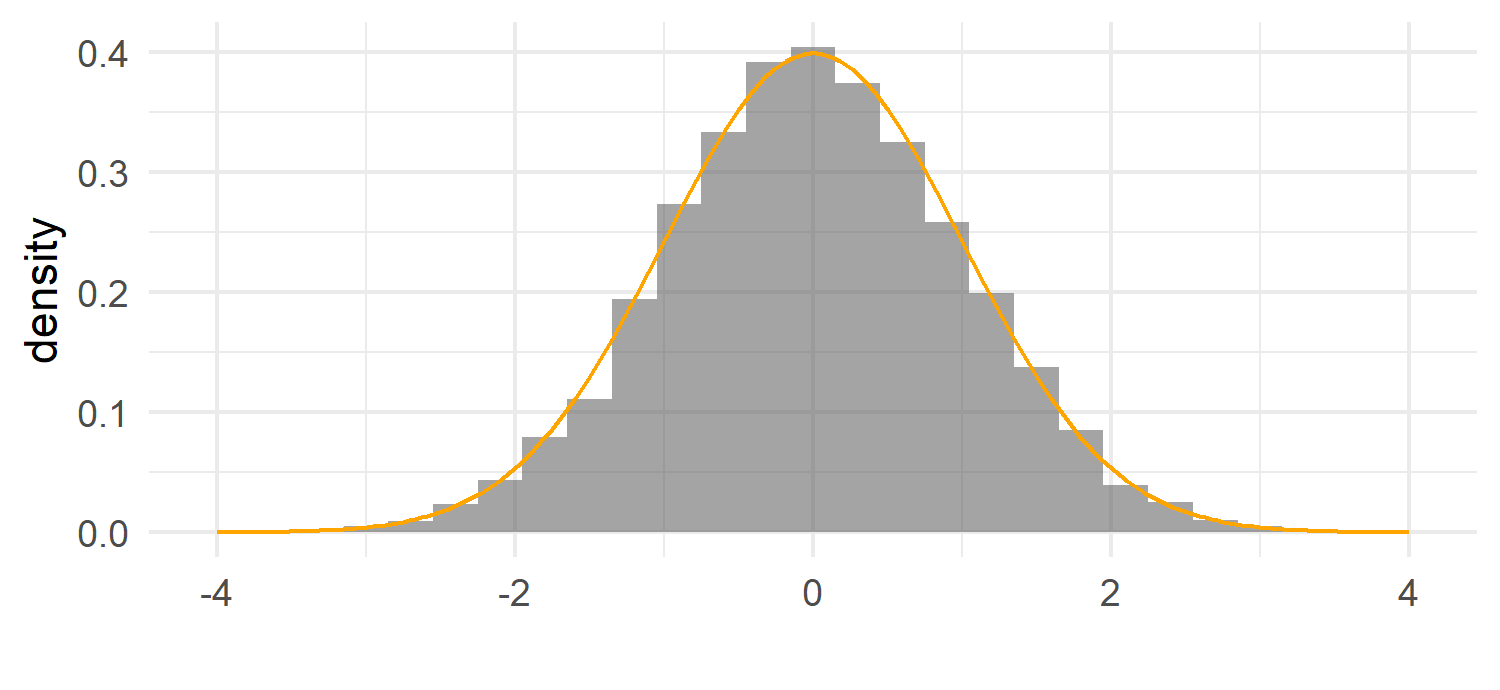
\includegraphics[width=0.8\textwidth, keepaspectratio]{ex2/normal_hist.png}
\caption{Histogram of simulated standard normals. The orange line shows the density of a standard normal variable}
\label{2normhist}
\end{figure}

Additionally one can examine the normality of a sample for example with QQ- and PP- plots. The QQ-plot for the sample is shown in Figure \ref{2normqq}. The points lie pretty much on the reference line. Just the few highest quantiles differ. Since on the tails are just a few data points this may happen by accident. I omit other plots since a very good fit of the data is already obvious in the histogram and the QQ- plot. 
\begin{figure}[bh]
\centering
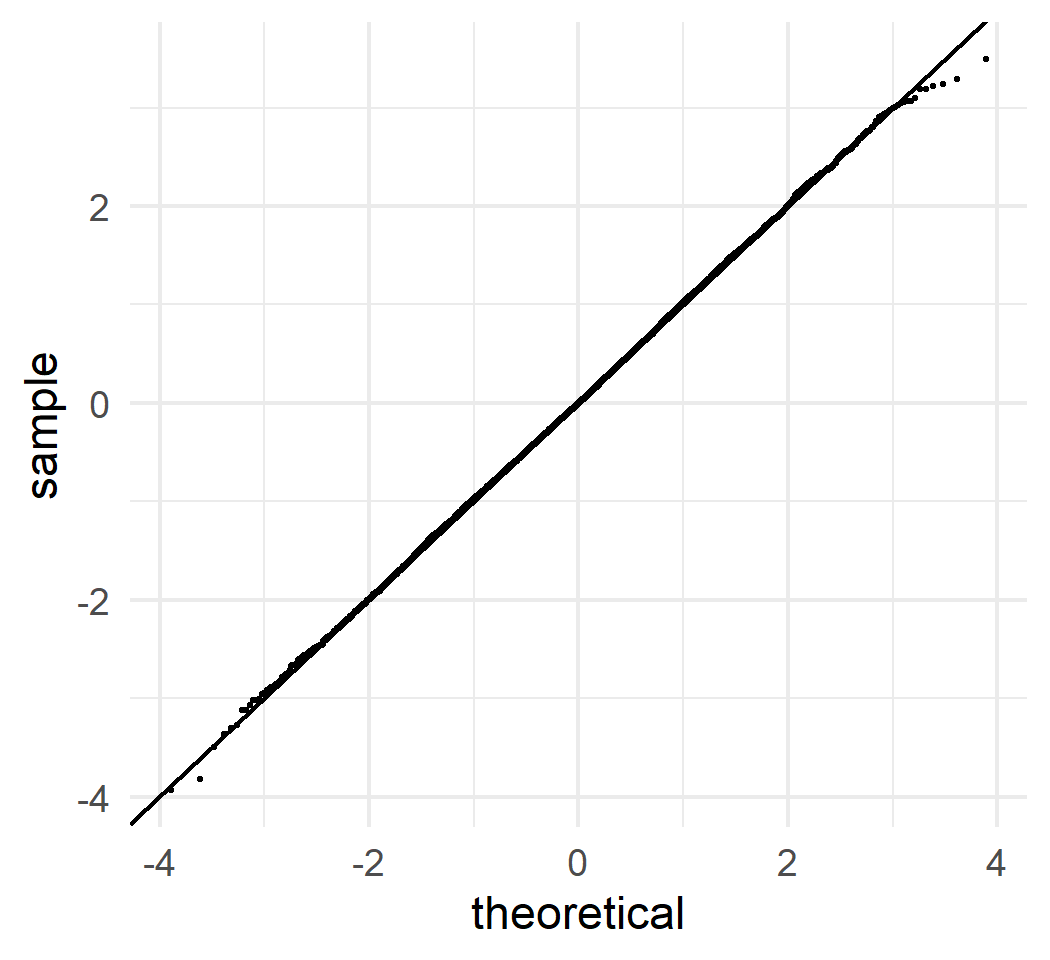
\includegraphics[width=0.45\textwidth, keepaspectratio]{ex2/normal_qq.png}
\caption{QQ-plot of a simulated sample of standard normals.}
\label{2normqq}
\end{figure}

Because in this method we reject some samples of the distribution $g$, it is interesting to consider the acceptance probability. The theoretical overall acceptance probability should be $1/c =0.658$. In this simulation we used 15 168 Cauchy samples resulting giving a similar empirical acceptance probability of $0.659$. One can also look in more detail and visualise more local acceptance probabilities. The probability that the uniform variable drawn in the second step of the algorithm accepts the sample $X$ as drawn from $f$ is $$P(U\leq \frac{f(X)}{cg(X)})=\frac{f(X)}{cg(X)}$$ and can be seen as a function in $X$. I estimated the local empirical acceptance probabilities by binning the data with the \texttt{hist} function in R (see Figure \ref{2normacc}). Since the Cauchy distribution has very heavy tails compared to the standard normal, there are of course very high and low values in the Cauchy sample. I restricted the data for the visualisation to the area, where the empirical acceptance probability is positive (and not 0), i.e. where we have indeed data in the final normal sample. As expected we see in the plot that the empirical probabilities fluctuate around the theoretical ones over the whole range of values.
\begin{figure}[hbt]
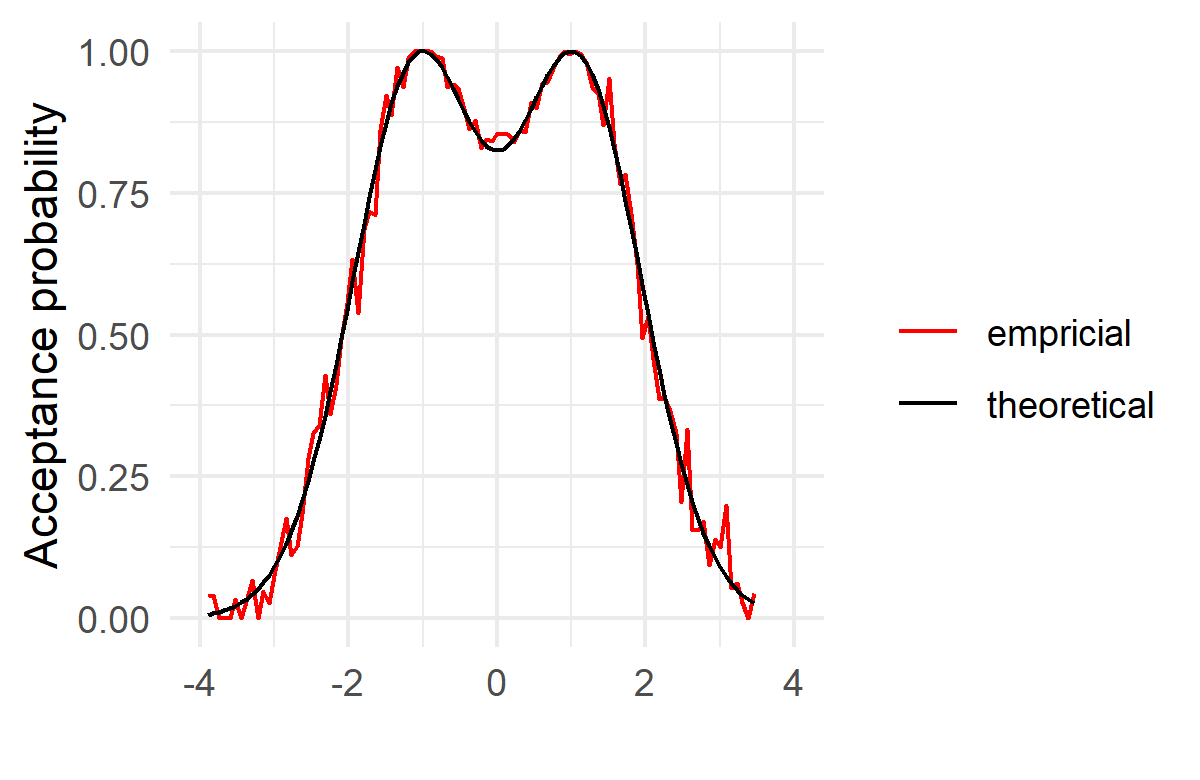
\includegraphics[width=0.7\linewidth, keepaspectratio]{ex2/acc_probs.png}
\centering
\caption{Theoretical and empirical acceptance probabilities of the normal sample generated with the accept-reject method.}
\label{2normacc}
\end{figure}

The last task of the exercise is to check, whether it is possible to simulate Cauchy distributed samples from a standard normal one. As mentioned the Cauchy distribution hat heavy tails compared to the normal. This can be also seen in the quotient of densities. $$\frac{g(x)}{f(x)}=\sqrt{2\pi}exp\{x^2/2\}[\pi (1+x^2)]^{-1}$$ This is obviously unbounded as $x$ tends to infinity, i.e. we can't find a suitable constant $c$ for the algorithm. This can also be seen in Figure \ref{2normacc}. As the limit of the function is 0 the inverse has to go to infinity.    